

\documentclass[letterpaper]{article}

\usepackage{hyperref}
\usepackage{geometry}
\usepackage{xspace}
\usepackage{graphicx}
\usepackage[T1]{fontenc}
\usepackage[sc,osf]{mathpazo}
\usepackage{amsmath}

\def\name{Jose Ignacio Castelli}
\def\footerlink{https://github.com/JicLotus/CV}

% PDF metadata
\hypersetup{
  colorlinks = true,
  urlcolor = black,
  pdfauthor = {\name},
  pdfkeywords = {android, software development, algorithms, computer science, mathematics},
  pdftitle = {\name: Curriculum Vitae},
  pdfsubject = {Curriculum Vitae},
  pdfpagemode = UseNone
}

\geometry{
  body={6.5in, 8.5in},
  left=1.0in,
  top=1.25in
}

% Page headers
\pagestyle{myheadings}
\markright{\name}
\thispagestyle{empty}

% Custom section fonts
\usepackage{sectsty}
\sectionfont{\rmfamily\mdseries\Large}
\subsectionfont{\rmfamily\mdseries\itshape\large}

% Don't indent paragraphs.
\setlength\parindent{0em}

% Make lists without bullets
\renewenvironment{itemize}{
  \begin{list}{}{
    \setlength{\leftmargin}{1.5em}
  }
}{
  \end{list}
}

\newenvironment{no-indent-itemize}{
  \begin{list}{}{
    \setlength{\leftmargin}{0em}
  }
}{
  \end{list}
}

\def\tilde{$\scriptstyle\sim$}
\def\bullet{$\circ$\xspace}

\begin{document}

{\huge \name}



\bigskip
\begin{minipage}{0.45\linewidth}
  \begin{tabular}{llll}
    
    
    Email: & \href{mailto:joseignaciocastelli92@gmail.com}{\tt joseignaciocastelli92@gmail.com} \\
     
    
    Github: &\href{http://github.com/jiclotus}{\tt http://github.com/jiclotus}\\
    
    Linkedin: &\href{https://www.linkedin.com/in/jose-ignacio-castelli-138763b0/}{\tt https://www.linkedin.com/in/jose-ignacio-castelli-138763b0/}\\
    
    Languages: & \textsc{en}, \textsc{es}\\
    Birth Date: & \textsc{07-18-1992}
    
    
  \end{tabular}
\end{minipage}


\hfill 
\smash{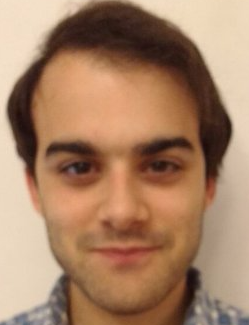
\includegraphics[width=3cm,height=3.5cm]{profilePic.png}}


\section*{Summary}
\begin{no-indent-itemize}
    \item Since I was thirteen years old I have been developing video games and company management systems in different languages. 
\end{no-indent-itemize}

\section*{Education}
\begin{no-indent-itemize}
  \item I hold a degree in Software Engineering from University of Buenos Aires 2011-2016 ( It is a 6-year university course equivalent to a Bachelor's and Master's degree) 
\end{no-indent-itemize}


\section*{Employment}
\begin{no-indent-itemize}

    \item\textsc{C\# .Net Developer at Supervielle Bank} | Jan 2017 - Present
    \begin{itemize}
    \item\bullet Billing management system in C\# , .Net framework and JS.
    \end{itemize}
    
    \item \textsc{C\# QR App} | Sep 2015 - May 2016
    \begin{itemize} 
    \item\bullet 
    This project was developed for coil control for a recycling plant. 
    \item\bullet Developed in C\#, Php and Android. 
    \end{itemize}
    \begin{itemize}
    \item
    Source \& Documentation:
    \href{https://github.com/JicLotus/Control-Sistematico-QR}{https://github.com/JicLotus/Control-Sistematico-QR}
    \end{itemize}


    \item\textsc{C++ Game Development} | Dec 2011 - Jul 2014
    \begin{itemize} \item\bullet
    This game was online with 167 players simultaneously. Now the game status is offline; however, it is under development. \href{https://www.facebook.com/InmortalAO/}{https://www.facebook.com/InmortalAO/}
    \end{itemize}

    \item\textsc{Visual Basic Game Development at NRG Games} | Jan 2008 - Jul 2008 
    \begin{itemize} \item\bullet
    My Second experience with another game Sponsor(NRG Games) in the development of Argentum Online 2D project. 
    \end{itemize}

    \item \textsc{Visual Basic Game Development at LocalStrike} | Jan 2007 - Dec 2007
    \begin{itemize} \item\bullet
    I had a game sponsor called LocalStrike for my Argentum Online 2D Game Project.
    \end{itemize}

\end{no-indent-itemize}


\section*{Projects}
\begin{no-indent-itemize}
    
    \item \textsc{3D WebGL Graphic Scene} | May 2016 - Jun 2016
    \begin{itemize}
    \item\bullet 3D graphic scene developed in WebGL and JS.
    \item\bullet Each vertex point in the graphic scene was positioned mathematically
    \end{itemize}
    \begin{itemize}
    \item Source \& Documentation: \href{https://github.com/JicLotus/3DGraphicScene}{https://github.com/JicLotus/3DGraphicScene}
    
    \end{itemize}

    \item \textsc{C++/Android Dropbox Open Source} | Aug 2015 - Dec 2015
    \begin{itemize}
        \item\bullet Dropbox open source for Android.
        \item\bullet The web server was developed in RocksDB in C++ language.
        \end{itemize}    
    \begin{itemize}
        \item Source \& Documentation:
        \href{https://github.com/JicLotus/Dropbox-source}{https://github.com/JicLotus/Dropbox-source}
    \end{itemize}

    \item \textsc{Capacitive touch sensors} |  Apr 2015 - Jul 2015

    \begin{itemize}
        \item\bullet Two capacitive touch sensors using an Atmega88pa microcontroller. These sensors were used for the control of intensity of a 12V light.
        
        Source \& Documentation: \href{https://github.com/JicLotus/Capacitive-Sensor}{https://github.com/JicLotus/Capacitive-Sensor}
    \end{itemize}

\end{no-indent-itemize}


\section*{Skills}
\begin{no-indent-itemize}
    
    \item\textsc{Main Programming Languages}: C\#, C++
    \item \textsc{Moderate Experience}: C, DirectX, OpenGL, WebGL, SDL, XNA, Php, Python, JAVA, SQL,Mysql,MSSql,MongoDB, Android, JS, Apache and Laravel.
    
\end{no-indent-itemize}


\bigskip
\begin{center}
  \begin{footnotesize}
    Last updated: \today \\
    \href{\footerlink}{\texttt{\footerlink}}
  \end{footnotesize}
\end{center}

\end{document}